% This file was created with tikzplotlib v0.10.1.post12.
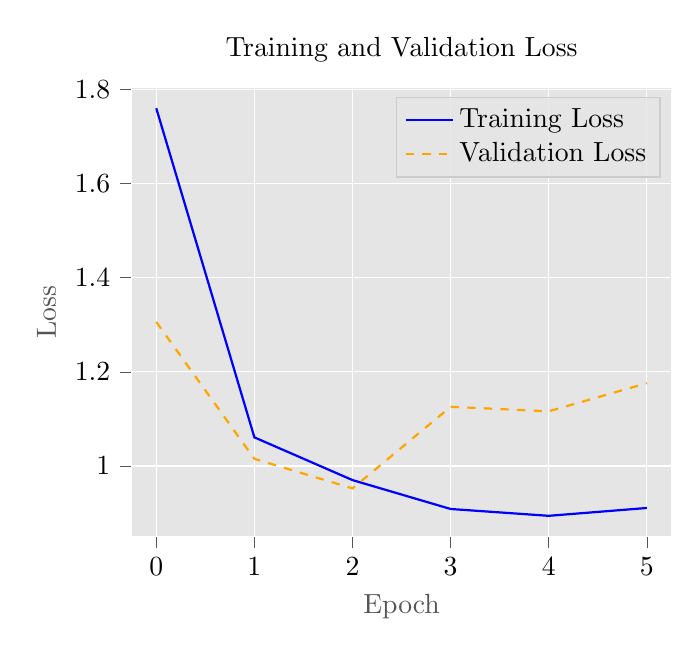
\begin{tikzpicture}

\definecolor{dimgray85}{RGB}{85,85,85}
\definecolor{gainsboro229}{RGB}{229,229,229}
\definecolor{lightgray204}{RGB}{204,204,204}
\definecolor{orange}{RGB}{255,165,0}

\begin{axis}[
axis background/.style={fill=gainsboro229},
axis line style={white},
legend cell align={left},
legend style={fill opacity=0.8, draw opacity=1, text opacity=1, draw=lightgray204, fill=gainsboro229},
tick align=outside,
tick pos=left,
title={Training and Validation Loss},
x grid style={white},
xlabel=\textcolor{dimgray85}{Epoch},
xmajorgrids,
xmin=-0.25, xmax=5.25,
xtick style={color=dimgray85},
y grid style={white},
ylabel=\textcolor{dimgray85}{Loss},
ymajorgrids,
ymin=0.850799956917763, ymax=1.80306544005871,
ytick style={color=dimgray85}
]
\addplot [thick, blue]
table {%
0 1.75978064537048
1 1.06072223186493
2 0.969964325428009
3 0.908586382865906
4 0.894084751605988
5 0.910750389099121
};
\addlegendentry{Training Loss}
\addplot [thick, orange, dashed]
table {%
0 1.30576848983765
1 1.01507687568665
2 0.952336370944977
3 1.12569200992584
4 1.11606097221375
5 1.17588150501251
};
\addlegendentry{Validation Loss}
\end{axis}

\end{tikzpicture}
